\chapter{Introduction}
The Internet is probably one of the most impacting inventions of all time. Nowadays, its infrastructure is the backbone of todays world and we have seen it: every time an issue occurs in the infrastracture, the damages are serious, both for economics and for human safety.

While Internet feels like magic to the ones that don't know it, it is much more appreciated by those who know well what is happening under the hood when we communicate over it.

In this tiny book, we will try to explain what is really happening when Alice and Bob (usually) talk over the Internet and also how they can securely talk when Tom (a malicious human being) tries to sneak between them to extract personal information or scam them.

Even though we will focus on the Internet, it is not the only existing \emph{computer network}: also your home router and your devices connected to it form a computer network -- a \emph{local} network --, which is part of a larger network that is the Internet -- a \emph{wide} network.

\section{History}
The foundations of modern computer networks and the Internet were laid in the 1960s with early research into packet-switching technology. Pioneering work by Leonard Kleinrock on packet-switching theory convinced researchers that data communications using discrete packets were far more robust than traditional circuit-switched telephone networks \cite{leiner1997past}. In 1969, the United States Department of Defense's Advanced Research Projects Agency (DARPA) commissioned the ARPANET, which connected its first nodes at UCLA and Stanford Research Institute.

As more distinct networks emerged, the challenge became interconnecting these disparate systems. The DARPA Internet architecture was specifically designed to solve this problem by multiplexing existing interconnected networks through gateways \cite{clark1988design}. The core design philosophy of this architecture—which ultimately became the TCP/IP protocol suite—prioritized survivability above all else. The system was built so that communications could continue seamlessly even if underlying network links or gateways failed. This resilient, decentralized foundation facilitated the explosive global growth of the network throughout the 1990s, evolving into the ubiquitous global infrastructure we now call the Internet \cite{leiner1997past}.

\section{Base Concepts}
Now, we are going to introduce some basic concepts of networks including their dictionary.

\subsection{Networks as Graphs}
We can very well describe a computer network through graphs: each connected device is a \keyword{node}, each connection between nodes is called \keyword{link} and a sequence of links is called a \keyword{path}.
In a simplified model, \emph{leaves}\footnote{Leaves are nodes that have one link at most.} such that a PC or a printer. Leaves are more commonly called \keyword{end-points}.

\subsection{Communication}
In general, a \keyword{communication} has five components:
\begin{itemize}
    \item A \keyword{message}: the data to communicate;
    \item A \keyword{sender}: \q{who}\footnote{This entity may not be a human being.} is sending the message;
    \item A \keyword{receiver}: \q{who} is supposed to receive the message;
    \item A \emph{medium}: the channel the message travels through;
    \item A \keyword{protocol}: a set of rules that both the sender and the receiver must know to properly exchange the message.
\end{itemize}

A communication is \keyword{connection-oriented} when it first ensures that the two hosts are connected -- via a \emph{handshake} -- before starting the actual message exchange, while it is \keyword{connectionless} when it happens without the previous preliminary exchange.
Moreover, a connection can be \keyword{persistent} or \keyword{non-persistent}: a persistent connection gets used for several communications, while a non-persistent one only serves a single communication.

A communication medium (or, more in general, a communication pattern) can be:
\begin{itemize}
    \item \emph{Simplex}: the node A can send messages to node B, but B cannot send messages to A: A is always the sender, B is always the receiver;
    \item \emph{Half-Duplex}: A and B can be both sender and receivers, but they must take turns: if A is sending a message to B, B cannot simultaneously send a message to A.
    \item \emph{Full Duplex}: A can send a message to B and B can simultaneously send a message to A.
\end{itemize}

We call \keyword{transmission rate} the maximum amount of data that a \emph{node} can trasmit.
\keyword{Bandwidth} is the maximum amount of data that a \emph{path} can trasmit, while the \keyword{throughput} is the actual amount of data that is being transmitted over a \emph{path}.
All these three, related metrics are measured in bits (or multiples) over seconds.

\subsection{Topology}
Every network has a \keyword{topology}, that is the arrangement of the nodes and their connections.
Typical topologies are:

\paragraph{Ring}
In a ring topology, each node is connected to exactly two other nodes, forming a continuous circular path. Data generally travels in a single direction. A failure in any individual link can potentially partition the entire network unless a dual-ring architecture is implemented.
\begin{center}
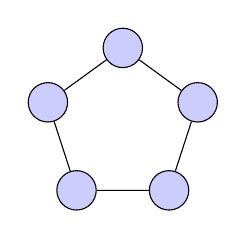
\begin{tikzpicture}[every node/.style={circle, draw, fill=blue!20, minimum size=0.5cm}]
\node (n1) at (90:1) {};
\node (n2) at (18:1) {};
\node (n3) at (306:1) {};
\node (n4) at (234:1) {};
\node (n5) at (162:1) {};
\draw (n1) -- (n2) -- (n3) -- (n4) -- (n5) -- (n1);
\end{tikzpicture}
\end{center}

\paragraph{Mesh}
A mesh topology features nodes interconnected with multiple other nodes, offering high redundancy and robust path selection. In a \emph{partial mesh}, only some nodes are interconnected, balancing cost and reliability.
\begin{center}
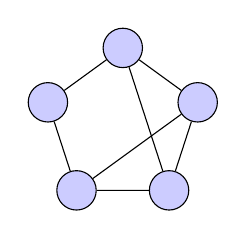
\begin{tikzpicture}[every node/.style={circle, draw, fill=blue!20, minimum size=0.5cm}]
\node (n1) at (90:1) {};
\node (n2) at (18:1) {};
\node (n3) at (306:1) {};
\node (n4) at (234:1) {};
\node (n5) at (162:1) {};
\draw (n1) -- (n2) -- (n3) -- (n4) -- (n5) -- (n1);
\draw (n1) -- (n3);
\draw (n2) -- (n4);
\end{tikzpicture}
\end{center}

\paragraph{Star}
The star topology connects all leaves (end-points) to a central centralizing node, such as a switch or hub. This design is highly manageable and isolates individual link faults well, but the central node represents a single point of failure.
\begin{center}
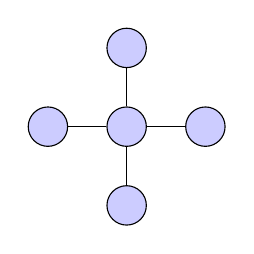
\begin{tikzpicture}[every node/.style={circle, draw, fill=blue!20, minimum size=0.5cm}]
\node (center) at (0,0) {};
\node (n1) at (90:1) {};
\node (n2) at (0:1) {};
\node (n3) at (270:1) {};
\node (n4) at (180:1) {};
\draw (center) -- (n1);
\draw (center) -- (n2);
\draw (center) -- (n3);
\draw (center) -- (n4);
\end{tikzpicture}
\end{center}

\paragraph{Fully Connected}
Also referred to as a full mesh topology, every single node in a fully connected network has a direct physical link to all other nodes. While providing the maximum possible redundancy, it scales quadratically, making it impractical for large networks.
\begin{center}
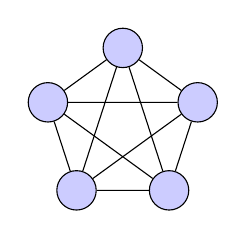
\begin{tikzpicture}[every node/.style={circle, draw, fill=blue!20, minimum size=0.5cm}]
\node (n1) at (90:1) {};
\node (n2) at (18:1) {};
\node (n3) at (306:1) {};
\node (n4) at (234:1) {};
\node (n5) at (162:1) {};
\draw (n1)--(n2) (n1)--(n3) (n1)--(n4) (n1)--(n5);
\draw (n2)--(n3) (n2)--(n4) (n2)--(n5);
\draw (n3)--(n4) (n3)--(n5);
\draw (n4)--(n5);
\end{tikzpicture}
\end{center}

\paragraph{Line}
A line (or daisy-chain) topology connects nodes sequentially. Messages must be passed through intermediate nodes to reach a destination. It is simple but vulnerable, as any link failure splits the network into two isolated segments.
\begin{center}
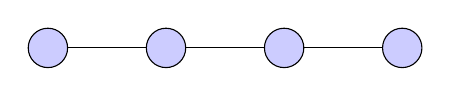
\begin{tikzpicture}[node distance=1.5cm, every node/.style={circle, draw, fill=blue!20, minimum size=0.5cm}]
\node (n1) at (0,0) {};
\node (n2) at (1.5,0) {};
\node (n3) at (3,0) {};
\node (n4) at (4.5,0) {};
\draw (n1) -- (n2) -- (n3) -- (n4);
\end{tikzpicture}
\end{center}

\paragraph{Tree}
A tree topology combines characteristics of star and line topologies, organizing nodes in a hierarchical structure with a root node cascading down to successive layers of child nodes. It is highly scalable and frequently used in both local and wide area networks.
\begin{center}
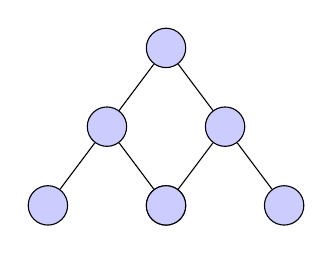
\begin{tikzpicture}[every node/.style={circle, draw, fill=blue!20, minimum size=0.5cm}, level distance=1cm, sibling distance=1.5cm]
\node {}
  child {node {}
    child {node {}}
    child {node {}}
  }
  child {node {}
    child {node {}}
    child {node {}}
  };
\end{tikzpicture}
\end{center}

\paragraph{Bus}
In a bus topology, all nodes share a single common communication medium (the backbone). A message broadcasted on the bus is physically heard by all nodes, but only processed by the intended receiver. It holds historic significance for early Ethernet deployments.
\begin{center}
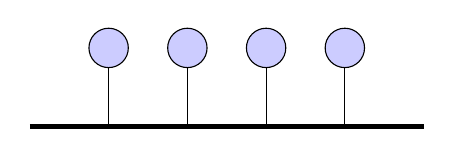
\begin{tikzpicture}[every node/.style={circle, draw, fill=blue!20, minimum size=0.5cm}]
\draw[ultra thick] (0,0) -- (5,0);
\node (n1) at (1,1) {};
\node (n2) at (2,1) {};
\node (n3) at (3,1) {};
\node (n4) at (4,1) {};
\draw (n1) -- (1,0);
\draw (n2) -- (2,0);
\draw (n3) -- (3,0);
\draw (n4) -- (4,0);
\end{tikzpicture}
\end{center}

\begin{example}{}
    Note that a computer network can have a physical topology that is different from the logical topology.
\end{example}

\begin{example}{Streaming a Movie over a LAN}
    Consider a scenario where a user on a local network wants to watch a movie streamed by a local server. We need to calculate the overall bandwidth of the path connecting the user's end-point to the server to determine if high-definition streaming is feasible. We assume a typical star topology for the home LAN: the media server and the smart TV are both connected to a central router. The media server connects to the router via a wired Ethernet link boasting a transmission rate of $1\text{ Gbps}$. The router's switch fabric is capable of forwarding data at $1\text{ Gbps}$. However, the smart TV is connected via a Wi-Fi link that has an effective transmission rate of $150\text{ Mbps}$. The bandwidth of the complete path is dictated by the bottleneck link; thus, the path bandwidth is $\min(1000\text{ Mbps}, 1000\text{ Mbps}, 150\text{ Mbps}) = 150\text{ Mbps}$. A high-definition (1080p) movie typically requires a throughput of around $5$ to $10\text{ Mbps}$, and a 4K movie demands about $25\text{ Mbps}$. Since the bottleneck bandwidth is $150\text{ Mbps}$, the network capacity comfortably supports high-definition playback.
\end{example}

\subsection{Network Scope}
Computer networks can be categorized based on the dimension of their scope: 
\begin{itemize}
    \item A \emph{Local Area Network} (\keyword{LAN}) typically does not cross the walls of a building; 
    \item A \emph{Wide Area Network} (\keyword{WAN}) is a network that extends over a large geographic area.
\end{itemize}

These two are only the most common classes. A richer classification is showed in \ref{img:network-scope-classification}.

\begin{figure}
    \centering
    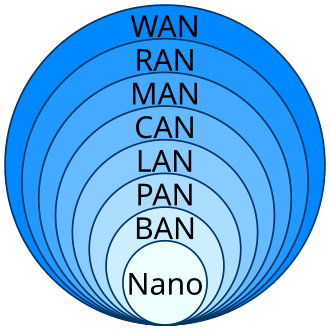
\includegraphics[width=0.3\textwidth]{_files/_images/network_scope_classification.png}
    \caption{Classification of computer networks based on their geographical scope, illustrating the spectrum from Personal Area Networks (PANs) spanning a few meters to Wide Area Networks (WANs) spanning the globe.}
    \label{img:network-scope-classification}
\end{figure}

\section{The Layered Architecture}
In \q{standard} networks, every node implements (partially or completely) a technological stack, that consists of layered softwares each of them implementing a specific communication protocol.
Each layer exposes an API to the upper layer and uses the services of the layer below.

The ISO Open System Interconnection (\keyword{ISO/OSI}) is the \emph{de iure} standard that defines seven layers of communication \cite{zimmermann1980osi}:
\begin{etaremune}
    \item \emph{Application Layer}. Protocols of this layer directly serve the end user by providing the distributed information service appropriate to an application. The other layers exist only to support this one;
    \item \emph{Presentation Layer}. This layer is the network's universal translator. While the lower layers worry about how to move data from point to point, the Presentation Layer worries about ensuring the data actually makes sense once it arrives.
        Encryption/decryption and compression/decompression are also handled in this layer;
    \item \emph{Session Layer}. This layer creates/tears down a connection -- a session -- between two presentation entities -- two systems at the Presentation Layer -- and defines the rules of data data exchange;
    \item \emph{Transport Layer}. If the session layer defines the rules of data exchange, this layer is the one that provides a transparent way to transfer data from a session entity to another, without knowing the actual network path the data will follow;
    \item \emph{Network Layer}. The purpose of this layer is to \emph{route} data through the network in the best possible way;
    \item \emph{Data Link Layer}. If the Network Layer is about finding the best route, the Data Link Layer is about node-to-node data transfer. The purpose of this layer is to trasmit data from one node to another.
    \item \emph{Physical Layer}. The Physical Layer provides mechanical, electrical, functional, and procedural characteristics to establish, maintain, and release physical connections (e.g., data circuits) between data link entities.
\end{etaremune}

Let's suppose that Alice, who has got an iPhone, wants to send a message to Bob, who has got an Android phone, via a live chat -- which is the network application (Application Layer). Assume this live chat creates a direct connection between the two clients, without a central server.

First, Alice and Bob's clients create a session (Session Layer) -- we will describe how in the next, more complete communication example.
Then, Alice's client compresses and encrypts the message (Presentation Layer) and handle it to the Session Layer, that will check against the previously defined communication rules and then pass the message to the Transport Layer.

The Transport Layer \emph{encapsulates} the message into a packet attaching the sender and receiver ports. Then, it handles the packet to the Network Layer.

The Network Layer encapsulates the Transport Layer packet into a Network Layer packet attaching the network addresses of the two hosts. Then, it handles this packet to the Data Link Layer.

The Data Link Layer performs a host-to-host data transfer inside a local network. At this layer, the Network Layer package gets encapsulated into another packet with the physical devices addresses attached. Then, the Data Link Layer communicates to the Pyhsical Layer this packet.

The Physical Layer is the layer that performs the physical data transfer through cables, radio waves etc.
Note that, at this point, the packet contains all the other packets like a Matrioska.

We will now overlook how this packet will finally reach Bob's device, but we will see this in depth in the following chapters. Just consider that the packet will be \emph{decapsulated} and encapsulated (up to the Network Layer) multiple times along the network path.

When the Physical Layer packet arrives to Bob's device, this device will decapsulate the packet and find a Data Link packet, that will decapsulate to find a Network packet and so on up to the Application Layer.

A layered approach like the OSI one allows great separation of concerns -- each layer can be updated without breaking (ideally) the other ones --, at the cost of a slower communication.
However, we will see some optimizations that require this layered approach to be less strict i.e. to allow some contamination between layers.

\begin{center}
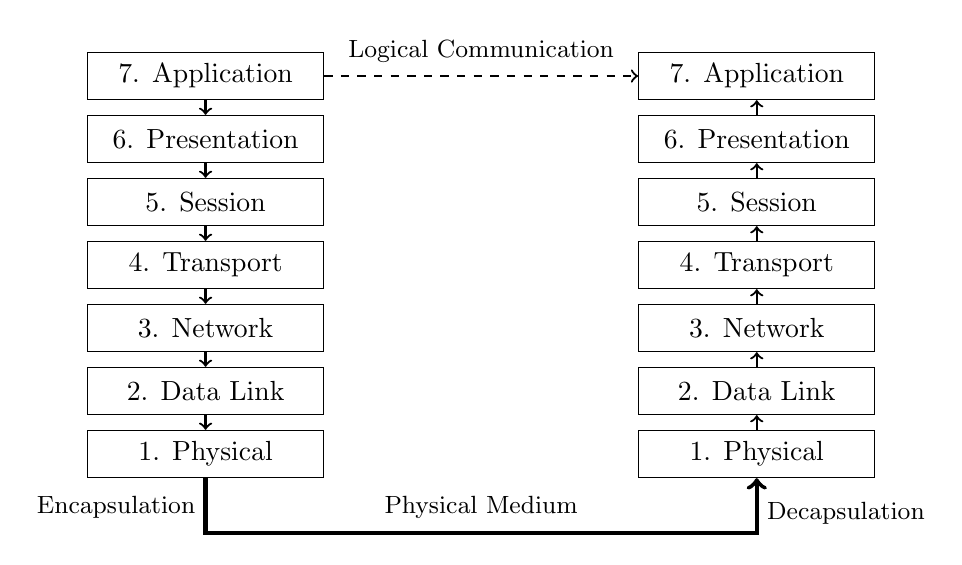
\begin{tikzpicture}[every node/.style={draw, minimum width=3cm, minimum height=0.6cm, align=center}, node distance=0.8cm]
\node (s7) at (0, 0) {7. Application};
\node (s6) at (0, -0.8) {6. Presentation};
\node (s5) at (0, -1.6) {5. Session};
\node (s4) at (0, -2.4) {4. Transport};
\node (s3) at (0, -3.2) {3. Network};
\node (s2) at (0, -4.0) {2. Data Link};
\node (s1) at (0, -4.8) {1. Physical};

\node (r7) at (7, 0) {7. Application};
\node (r6) at (7, -0.8) {6. Presentation};
\node (r5) at (7, -1.6) {5. Session};
\node (r4) at (7, -2.4) {4. Transport};
\node (r3) at (7, -3.2) {3. Network};
\node (r2) at (7, -4.0) {2. Data Link};
\node (r1) at (7, -4.8) {1. Physical};

\draw[->, thick, dashed] (s7.east) -- node[above, draw=none, minimum width=0cm, font=\small]{Logical Communication} (r7.west);

\draw[->, thick] (s7.south) -- (s6.north);
\draw[->, thick] (s6.south) -- (s5.north);
\draw[->, thick] (s5.south) -- (s4.north);
\draw[->, thick] (s4.south) -- (s3.north);
\draw[->, thick] (s3.south) -- (s2.north);
    \draw[->, thick] (s2.south) -- node[left, draw=none, minimum width=0cm, font=\small, pos=6.3]{Encapsulation} (s1.north);

    \draw[->, thick] (r1.north) -- node[right, draw=none, minimum width=0cm, font=\small, pos=-5.7]{Decapsulation} (r2.south);
\draw[->, thick] (r2.north) -- (r3.south);
\draw[->, thick] (r3.north) -- (r4.south);
\draw[->, thick] (r4.north) -- (r5.south);
\draw[->, thick] (r5.north) -- (r6.south);
\draw[->, thick] (r6.north) -- (r7.south);

\draw[->, ultra thick] (s1.south) -- (0, -5.8) -- node[above, draw=none, minimum width=0cm, font=\small]{Physical Medium} (7, -5.8) -- (r1.south);
\end{tikzpicture}
\end{center}

Logically, two nodes communicate at the same layer, making use of the layers below transparently.

\begin{note}{}
    Typically, only endpoints implement the whole stack: a network router strictly needs to implement up to level 3.
    This is another, very useful gain of using a layered architecture.
\end{note}

While the OSI model, standardized by the ISO, serves as the \emph{de iure} standard and the definitive reference architecture for understanding networking layers, it is the TCP/IP protocol suite that historically became the \emph{de facto} standard of the Internet \cite{clark1988design}. The DARPA-funded TCP/IP stack won the \q{protocol wars} largely due to its pragmatic, working implementations and its highly resilient design philosophy. However, modern network engineering often conceptualizes systems using a hybrid five-layer model that blends OSI's rigid abstractions with TCP/IP's practical protocols. 

In these notes, we will follow the very same top-down approach of Kurose et al.~\cite{kurose2017}.

\section{The Internet Community}
The Internet is not owned or controlled by any single entity. Instead, its development and governance are managed by a decentralized, global community of researchers, network operators, equipment vendors, and enthusiasts. This community collaborates to propose, discuss, and define the protocols and standards that make the Internet work.

At the core of Internet standardization is the \emph{Internet Engineering Task Force} (\emph{IETF}) \cite{rfc3935}. Founded in 1986, the IETF is the premier standards development organization for the Internet. It is responsible for producing the technical and engineering documents that influence how people design, use, and manage the network. The IETF operates under the famous mantra of \q{rough consensus and running code} \cite{rfc3935}: rather than relying on formal voting, standards are built on the combined engineering judgment of its participants and their real-world experience in implementing specifications.

The IETF publishes its standards and protocols in a series of documents known as \emph{Request for Comments} (\emph{RFC}s). The process by which an idea becomes an Internet standard is thoroughly documented in RFC 2026 \cite{rfc2026}. Anyone can participate in the IETF by joining open mailing lists or attending meetings, ensuring an open and transparent standard-setting process. 

The IETF is managed by the \emph{Internet Engineering Steering Group} (\emph{IESG}), which oversees the various working groups where the actual protocol development happens. Furthermore, the \emph{Internet Architecture Board} (\emph{IAB}) provides long-term technical direction and architectural oversight for the Internet. The IAB also oversees the \emph{Internet Research Task Force} (\emph{IRTF}), which focuses on long-term research topics related to Internet protocols, applications, and technology, leaving the short-term engineering issues to the IETF.

All of these organizations operate under the umbrella of the \emph{Internet Society} (\emph{ISOC}), a non-profit organization founded in 1992 to provide an institutional home and financial support for the Internet standards process.

While the IETF handles the core protocols of the Internet (such as TCP/IP, routing protocols, and DNS), other standard organizations play crucial roles in networking:
\begin{itemize}
    \item \emph{IEEE} (Institute of Electrical and Electronics Engineers): Defines standards for the lower layers of the network architecture, such as physical connections and data link protocols (e.g., IEEE 802.3 for Ethernet and IEEE 802.11 for Wi-Fi).
    \item \emph{W3C} (World Wide Web Consortium): Develops standards for the World Wide Web, including HTML, CSS, and XML.
    \item \emph{ICANN} (Internet Corporation for Assigned Names and Numbers): Coordinates the global allocation of IP addresses and manages the root of the Domain Name System (DNS).
\end{itemize}
